\section{Intelligence Artificielle}

\subsection{Stratégies}

\subsubsection{Intelligence aléatoire}
Cette stratégie consiste en un joueur qui a chaque étape du jeu aurait le choix entre plusieurs options et en choisit une de manière aléatoire.

\subsubsection{Intelligence Heuristique}
Dans l'intelligence heuristique, l'IA devra avoir un meilleur comportement qu'avec les commandes générées par le hasard. Ainsi, les choix faits par l'IA seront davantage réfléchis et permettront d'avancer d'une meilleure manière vers la fin du jeu et la défaite ou la victoire de l'un des deux joueurs. 
Pour chaque fonction, il est clair que de nombreuses stratégies existent pour joueur au Risk, que, dans une partie réelle, plusieurs d'entre-elles s'entremêlent inévitablement pour apporter le meilleur résultat possible au joueur. Dans notre cas, nous choisissons et expliquons une stratégie envisageable, réalisable pour notre jeu.
\newline


\begin{itemize}
    \item \textbf{aiRepartitionArmees.} 
    Dans cette fonction, l'IA doit choisir combien d'armées elle place sur chacun des territoires qui lui sont attribués. Pour trouver la meilleure méthode et stratégie, il convient de rappeler l'objectif du jeu. Pour l'instant, conquérir une certaine partie de la carte est l'objectif fixé : disons que le joueur gagnant devra posséder 25 territoires pour gagner (donc en conquérir 11). L'idée est donc de placer le plus d'armées sur les territoires qui ne sont pas trop isolés. En effet, posséder un réseau de pays sur lesquels les déplacements sont possibles permet de mieux structurer son attaque, effectuer des déplacements, mais aussi organiser sa défense.
    \newline
    
    \item \textbf{aiChoixPaysAttaquant.}
    Dans cette fonction, l'intelligence artificielle devra choisir le pays qu'elle possède avec le plus d'armées afin d'attaquer. Si plusieurs pays ont le même nombre d'armées, elle devra sélectionner celui qui est le plus en contact avec des états voisins appartenant au même joueur. Là encore, cette méthode permettra de renforcer les éventuelles pertes ou de ré-organiser la mise en place des armées en cas de défaite de l'attaque. 
    \newline
    
    \item \textbf{aiChoixPaysAttaque.}
   De manière très simple, nous choisissons d'attaquer le pays frontalier ennemi qui a le plus moins d'armées possible. Cela donne un pourcentage de chance plus important de remporter une attaque, et un éventuel territoire. Si plusieurs pays frontaliers ont le nombre d'armées minimum, on choisit le pays qui a le plus de frontaliers appartenant au joueur.
   %j'ai changé j'ai mis l'inverse de ce que tu avais mis
   \newline
   
   \item \textbf{aiNombreLancersAttaque.}
    On rappelle que l'attaque ne peut pas attaquer en mettant en péril son territoire. De plus, le choix du nombre d'armées attaquantes, et de défense se fait en même temps, ainsi aucun des deux joueurs ne peut connaître le choix fait par son adversaire avant de choisir à son tour. 
    \newline
    L'attaquant peut choisir d'attaquer avec 1, 2 ou 3 armées. Lorsque c'est possible, le mieux est bien entendu d'attaquer avec trois armées puisque cela augmente la possibilité de réaliser un bon lancer de dés. Lorsque le joueur attaquant possède 4 armées ou plus, il choisit d'attaquer avec 3 armées. Si l'attaquant possède 3 armées sur le territoire, il attaque avec 3 armées si le pays attaqué dispose de 2 armées ou moins pour défendre. Sinon, il attaque avec 2 armées. Si l'attaquant possède 2 armées, il attaque avec 1 si le pays attaqué dispose de 2 armées ou plus, sinon il attaque avec 2. 
    \newline
    
    \item \textbf{aiNombreLancersDefense.}
    Dès que possible, l'IA défend avec 2 armées. Cela augmente ses chances de battre l'attaque, bien que le risque de perdre deux pions soit aussi présent. 
    Si le défenseur possède 1 ou 2 armées sur le territoire, il défend avec 1. 
    Si le défenseur possède plus de 2 armées, et que le pays attaquant dispose de moins de 10 armées, il défend avec 2, sinon avec 1. 
    % Pourquoi les 10 armées ? au pif, on peut mettre autre chose hihi
    \newline
    
    \item \textbf{aiPlacerNouvellesArmees.}
    Lorsque le joueur doit placer de nouvelles armées à la fin de son tour, il choisit de les placer sur ses territoires possédant le moins d'armées.
    \newline
    
    \item \textbf{aiDéplacerArmées.}
    Plusieurs déplacements sont très intéressants à effectuer. Si le joueur possède un territoire entièrement entouré par des territoires amis, alors on ne peut laisser qu'une unique armée dessus (attaque impossible dessus) et ainsi renforcer les défenses alentours. 
    Par ailleurs, il peut être intéressant de renforcer des pays qui ne possèdent pas beaucoup d'armées. Si jamais un pays possède plus de 4 armées, et qu'un de ses voisins ne possède plus qu'1 ou 2 armées, alors nous ferons un déplacement de 1 ou 2. Dans un soucis de facilitation du code, nous ne regarderons que les voisins directs. 
    \newline
    
    
\end{itemize}

\newpage
\subsection{Conception logiciel}
Le diagramme des classes pour l’intelligence artificielle est présenté en figure \ref{fig:ai}.

\textbf{Les Classes AI} : Les classes héritières de AI implémente plusieurs stratégies d'intelligence artificielle.
\begin{itemize}
    \item RamdomAI : Intelligence aléatoire
    \item HeuristicAI : Intelligence heuristique
\end{itemize}

\begin{landscape}
    \begin{figure}[!htbp]
        \centering
        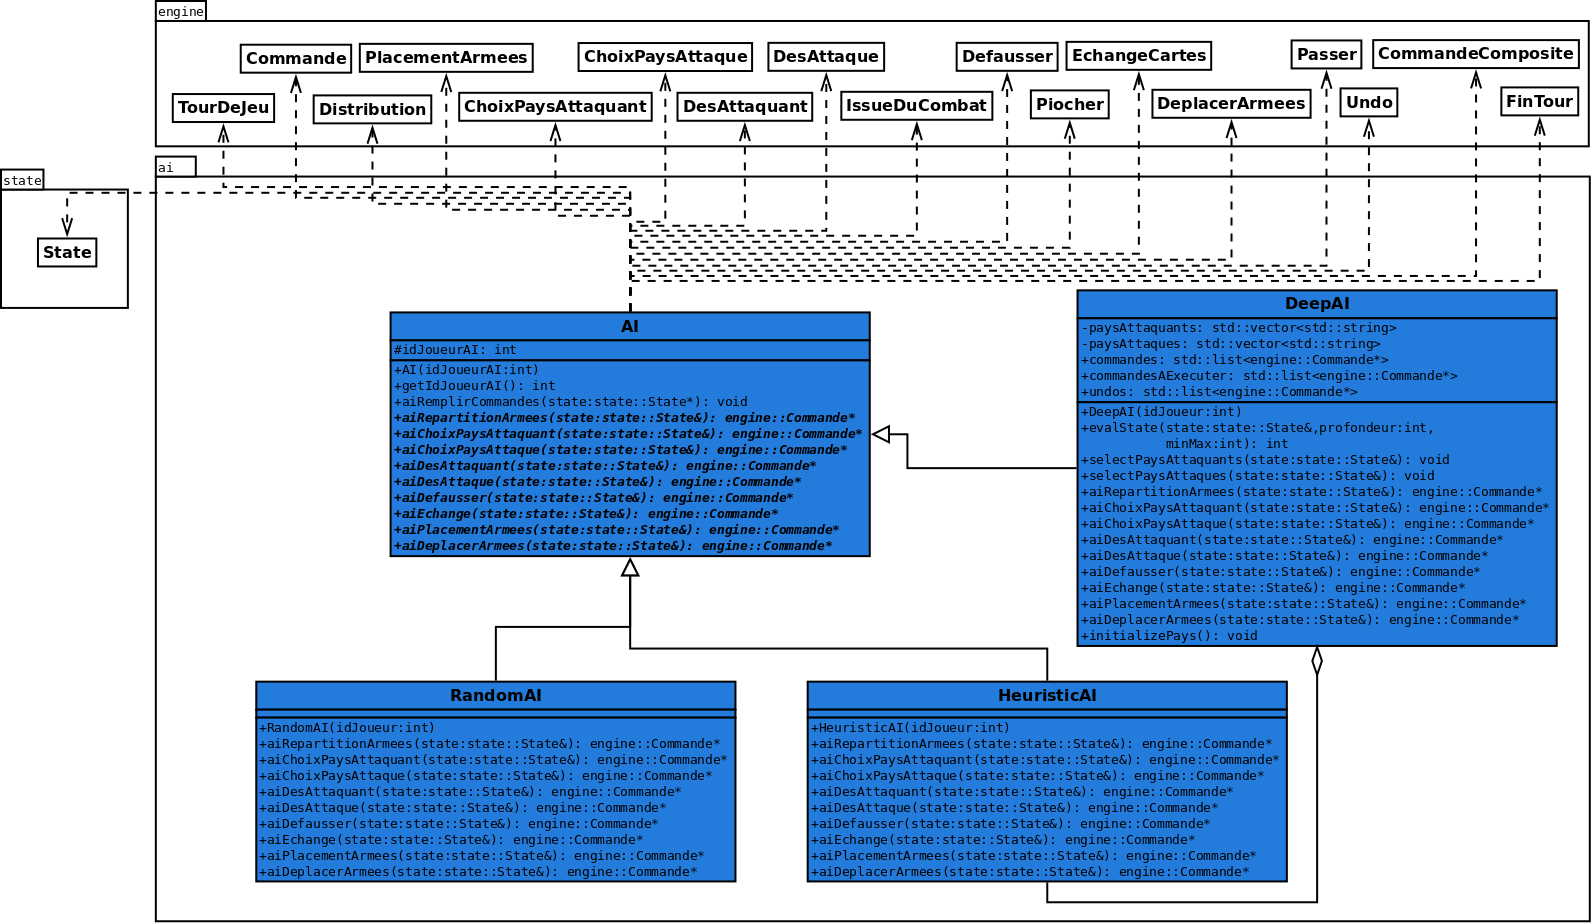
\includegraphics[width=17cm]{Images/ai.png}
        \caption{Diagramme de l'intelligence artificielle}
        \label{fig:ai}
    \end{figure}
\end{landscape}



\subsection{Liste des commandes}
\begin{itemize}

\item \textbf{random ai}
\newline
Touche espace : répartition des pays
\newline
Touche P : l'ai random joue seule 
\newline
Touche C : ai random tour 0 
\newline
Touche V : ai random tour par tour après avoir pressé C. 
\newline 
\newline
\item \textbf{heuristic ai}
\newline
Touche espace : répartition des pays
\newline
Touche P : l'heuristic joue seule 
\newline
Touche C : Heuristic tour 0 
\newline
Touche V : Heuristic tour par tour après avoir pressé C. 
\newline 
\newline



\end{itemize}

